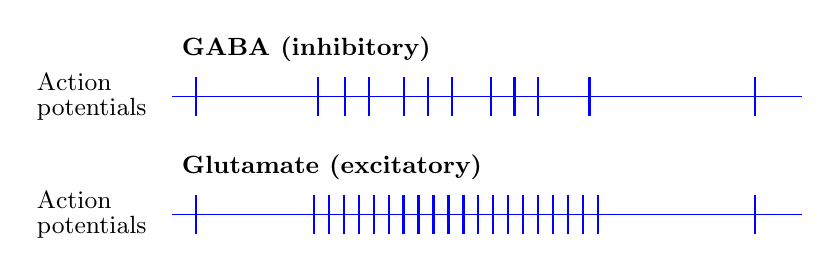
\begin{tikzpicture}[
  rowlab/.style={font=\small, align=left, anchor=east},
  spike/.style={blue, thick}
]
% GABA: few action potentials
\node[font=\small\bfseries, anchor=west] at (0,2.1) {GABA (inhibitory)};
\node[rowlab] at (-0.2,1.5) {Action\\[-2pt]potentials};
\draw[blue] (0,1.5) -- (8,1.5);
\foreach \x in {0.3,1.85,2.2,2.5,2.95,3.25,3.55,4.05,4.35,4.65,5.3,7.4} {
  \draw[spike] (\x,1.25) -- (\x,1.75);
}
% glutamate: many action potentials
\node[font=\small\bfseries, anchor=west] at (0,0.6) {Glutamate (excitatory)};
\node[rowlab] at (-0.2,0) {Action\\[-2pt]potentials};
\draw[blue] (0,0) -- (8,0);
\draw[spike] (0.3,-0.25) -- (0.3,0.25);
\foreach \i in {0,...,19} {
  \pgfmathsetmacro{\x}{1.8+0.19*\i}
  \draw[spike] (\x,-0.25) -- (\x,0.25);
}
\draw[spike] (7.4,-0.25) -- (7.4,0.25);
\end{tikzpicture}
